\documentclass{beamer}
%\pgfpagesuselayout{2 on 1}[a4paper,portrait,border shrink=5mm]
%\pgfpagesuselayout{8 on 1}[a4paper,portrait,border shrink=5mm]

\usepackage{../fhnw-beamer}

\date{\today}
\author{rolf.schmutz@fhnw.ch}
\institute{FHNW}
\title {Netzwerke und Datenkommunikation}

\usepackage{verbatim}
\usepackage{amsmath}
\usepackage{yfonts}

\begin{document} % ===============================================================


\begin{frame}
\frametitle{Empfohlene Links}
\begin{itemize}
  \item Google Video-Kurs (5h!) \myurl{https://www.youtube.com/watch?v=QKfk7YFILws}
  \item Netz-Mafia Grundlagen: \myurl{http://www.netzmafia.de/skripten/netze/index.html}
  \item Netz-Mafia Internet: \myurl{http://www.netzmafia.de/skripten/internet/index.html}
\end{itemize}

\begin{tiny}

\begin{itemize}
  \item routing is done on a next-hop basis
  \item ARP
  \item L3 allows every device to determine if a destination is {\em local} or {\em remote} (and only reachable via gateway)
  \item picture of a whole lot of intermediate L3/router with seperate L2 in-between
\end{itemize}
\end{tiny}
\end{frame}



\section{ND04: IP Layer-3}
\subsection{\"Ubersicht}

\begin{frame}
\frametitle{L3: Lenrziele}
\begin{itemize}
	\item{Sie kennen die Unterschiede Layer-2 zu Layer-3 Adressierung}
	\item{Sie kennen die Strukturierung der Layer-3 Adressen in (Sub-) Netze}
	\item{Sie wissen, dass IP/Layer-3 ein {\em paketvermittelndes} Netz darstellt}
	\item{Sie verstehen das Konzept der {\em Netzmasken} und k\"onnen es anwenden}
	\item{Sie wissen wie Layer-3 Pakete {\em geroutet}\footnote{Wegleitung im Internet}werden}
	\item{Sie wissen, dass IP/Layer-3 nach dem {\em best-effort} Prinzip arbeitet und die Zustellung der Pakete nicht garantiert ist}
	\item sie kennen ARP und ICMP und k\"onnen die grundlegende Funktion erkl\"aren
\end{itemize}
\end{frame}




\begin{frame}
\frametitle{L2 revisited: Intermediate Device Operation (Bridge) (1/4)}
\begin{figure}
\centering
\includegraphics[width=12cm]{L2_intermediate-device}
\end{figure}
\end{frame}


\begin{frame}
\frametitle{L2 revisited: LAN-extension (same LAN) (2/4)}
\begin{centering}
\includegraphics[width=12cm]{L2-base-network.pdf}
\end{centering}
\end{frame}

\begin{frame}
\frametitle{L2 revisited: ``Internet'' with L2? (3/4)}
\includegraphics[width=10cm]{L2-base-network-L2-gateway.pdf}
\end{frame}

\begin{frame}
\frametitle{L2 revisited: L2-``Internet'' Problems  (4/4)}
\begin{itemize}
  \item die CAM/Port-Tabelle w\"achst bei Erweiterung des Netzwerks potentiell bis zur Anzahl Hosts
  \item ein weltweites Internet ist so nicht realisierbar: die CAM-Tabelle w\"urde alle potentiellen Ziele im Internet unter dem ``Uplink''-Port speichern
  \item einfach alles unbekannte per ``Flooding'' auf den Uplink schicken funktioniert ebenfalls nicht:
    \begin{itemize}
      \item ein weltweites Internet w\"urde nur duch das Flooding ausgelastet
      \item zudem k\"onnte alle Hosts mith\"oren (der ``privater Link'' Vorteil geht verloren)
    \end{itemize}
\end{itemize}
\begin{block}{}
MAC-Adressen sind {\em Ger\"ateadressen} (Device-Address) und haben keine strukturelle Lokalisierung/Gruppenzusammengeh\"origkeit

\begin{center}LAN = ``Just a bunch of devices''\end{center}
\end{block}
\end{frame}

\begin{frame}
\frametitle{L2: the need for L3 :) (1/2)}
\begin{itemize}
  \item Hosts/Ger\"ate m\"ussen in einer lokalisierten Gruppe zusammengefasst werden: ``logische'' (abstrakte) Adressierung
  \item {\em forwarding}/Weiterleitung Aufgrund der Gruppe (``Netz'') und nicht der einzelnen Ger\"ateadressen $\rightarrow$ viel kleinere ``Routingtabellen''
\end{itemize}
\vspace{-0.2cm}
\begin{figure}{}
  \centering
  \includegraphics[width=8cm]{L2-base-network-L3-gateway.pdf}
\end{figure}
\end{frame}


\begin{frame}
\frametitle{L2: the need for L3 (2/2)}
\begin{itemize}
  \item Die IP-Adressierung ist vergleichbar mit den Telefonnummern: zuerst die globale Vorwahl, Ortsvorwahl und dann die Apparatennummer
    \begin{itemize}
      \item Die Adressen sind so strukturiert, dass die ``Ger\"ate''/Hosts {\em rechts} nummeriert werden
      \item die ``Vorwahl''/Gruppe ist {\em links} gehalten
    \end{itemize}
\end{itemize}
\begin{block}{}
Die Adressen sind in der Regel {\em ortsgebunden} (localized) und werden auf die Ger\"ate {\em konfiguriert}\footnote{im Gegensatz zu den MAC/L2-Adressen, die fest eingestellt sind. Das kann automatisch (DHCP) oder manuell erfolgen}
\end{block}
\begin{itemize}
  \item ein L2-Netzwerk kann beliebig viele L3-Gruppen (Netze) enthalten\footnote{d.h. L2 funktioniert unabh\"angig von L3}, das stiftet aber in der Regel Verwirrung :)
\end{itemize}
\end{frame}


%%%%%%%%%%%%%%%%%%%%%%%%%%%%%%%%%%%%%%%%%

\begin{frame}
\end{frame}

\frametitle{L3 Stack}
\includegraphics[width=12cm]{stack-overview-3}

Header:
\begin{itemize}
  \item{\emph{global} g\"ultige \emph{End-zu-End} (Ger\"ate) Adressierung}
  \item{\emph{Header}-Pr\"ufsumme\footnote{d.h. keine Pr\"ufsumme \"uber die SDU}}
  \item{Flags, Fragment, ``Lebensdauer'', Unters\"utzung f\"ur (einfache) Qualit\"atsicherung etc}
  \item{\ldots und nat\"urlich das ``upper-level-protocol''}
\end{itemize}
\end{frame}

\begin{frame}
\frametitle{L3 Factlets}
\begin{itemize}
	\item{Layer-3 verbindet Systeme {\em End-to-End} \footnote{im Gegensatz zu Layer-2, das nur Teilstrecken/benachbarte Systeme verbindet} -- d.h. weltweit}
	\item{Layer-3 Adressen sind {\em strukturiert} in (Sub-) Netze\footnote{wie z.B. das Telefon-Netzwerk}}
	\item{IP/Layer-3 ist ein {\em paketvermittelndes} Netz: die Nutzdaten werden paketisiert und gesondert \"ubertragen}
	\item{verschiedene Layer-3 Netzwerke werden durch {\em Router}\footnote{oder ``Gateway'' (ungenauer)} miteinander verbunden}
	\item{die Dateneinheit auf IP/Layer-3 ist das Paket ``packet''\footnote{bei Layer-2 war das ``frame''}}
	\item{die Zustellung der Pakete auf IP/Layer-3 ist nicht garantiert\footnote{im Gegensatz zu Ethernet/L2 kann aber L3 bereits Fehlermeldungen zum Kommunikationspartner ausl\"osen -- \emph{wenn} die Header-Checksum stimmt\ldots}}
\end{itemize}
\end{frame}

\begin{frame}
\frametitle{Paketvermittelndes Netz}
\begin{itemize}
	\item{Layer-3 unterteilt die Nutzdaten\footnote{z.B. Webseiten oder Bild- und Tondaten} in kleinere Einheiten und versendet diese gesondert \"uber das Netz\footnote{wie auch schon auf Layer-2}}
	\item{Die Pakete k\"onnen verloren gehen oder in anderer Reihenfolge\footnote{oder auch {\em verdoppelt} werden} am Ziel ankommen -- die Wiederherstellung der Nutzdaten ist Aufgabe der oberen Layer}
	\item{ein paketvermittelndes Netz ist Fehlerresistent\footnote{solange die oberen Layer f\"ur die garantierte Zustellung aufkommen. Der Ausfall einzelner Verbindungen/L2 im Internet ist \"ublicherweise kein Problem}}
	\item{\ldots und erlaubt eine effiziente Auslastung\footnote{im Gegensatz zu leitungsvermittelnden Netzen -- wo die Reservierung der Bandbreite unabh\"angig der tats\"achlichen Ausnutzung erfolgt} der Resourcen}
\end{itemize}
\end{frame}




\begin{frame}
\frametitle{Unterschiede Layer-2 zu Layer-3 Adressierung}
\begin{itemize}
	\item{Layer-2 ist eine {\em Ger\"ate-Identifikation}\footnote{wie z.B. die AHV-Nummer} {\em ohne} Struktur/Lokationsinformation}
	\item{ein Internet\footnote{weltweiter Netzwerkverbund} w\"are mit Layer-2 Adressen nicht m\"oglich, da die Bridge-Tabellen zu gross w\"urden}
	\item{Layer-3/IP fasst mehrere Ger\"ate in einem IP-(Sub-) Netz zusammen\footnote{wie bei den Telefonnummern die Landesvorwahl/Ortsvorwahl} und erlaubt so eine effiziente lokalisierung}
	\item{\"uber Layer-3/IP ist so eine weltweite lokalisierung/addressierung von {\em Endger\"aten} m\"oglich}
\end{itemize}
\end{frame}

\begin{frame}
\frametitle{L3 Intermediate Device Operation (Router)}
\begin{figure}{}
\centering
\includegraphics[width=12cm]{L3_intermediate-device}
\end{figure}
\end{frame}

\begin{frame}
\frametitle{L3 end-to-end}
\begin{figure}
\centering
\includegraphics[width=12cm]{L3_multiple_L2}
\end{figure}
\end{frame}




\begin{frame}
\frametitle{Struktur der IP-Adressen (1/3)}
\begin{itemize}
  \item IP-Adressen werden wie Telefonnummern von links nach rechts ``spezifischer'':
  \begin{itemize}
    \item links ist die globale Einordnung: ``Vorwahl'' (prefix)
    \item rechts ist der einzelne Anschluss/Apparat
  \end{itemize}
  \item ``Routing'' basiert nur auf dem ``Vorwahl''-Teil\footnote{d.h. weit entfernte Router brauchen nur den Prefix und nicht die vollst\"andige Adresse}, es muss eine effiziente\footnote{weil {\em jedes} Paket aufs Neue ``geroutet'' wird} Methode zur ``Extraktion'' des Prefix gefunden werden
\end{itemize}
\end{frame}

\begin{frame}
\frametitle{Struktur der IP-Adressen: Prefix/Netz-Anteil (2/3)}
\begin{itemize}
	\item{IPv4-Adressen sind 32-Bit breit und werden \"ublicherweise im ``dotted-decimal''\footnote{4-Bytes im Dezimalformat 0-255 getrennt durch ``.''} Format notiert: {\texttt 194.41.161.1}}
\end{itemize}
  {\center 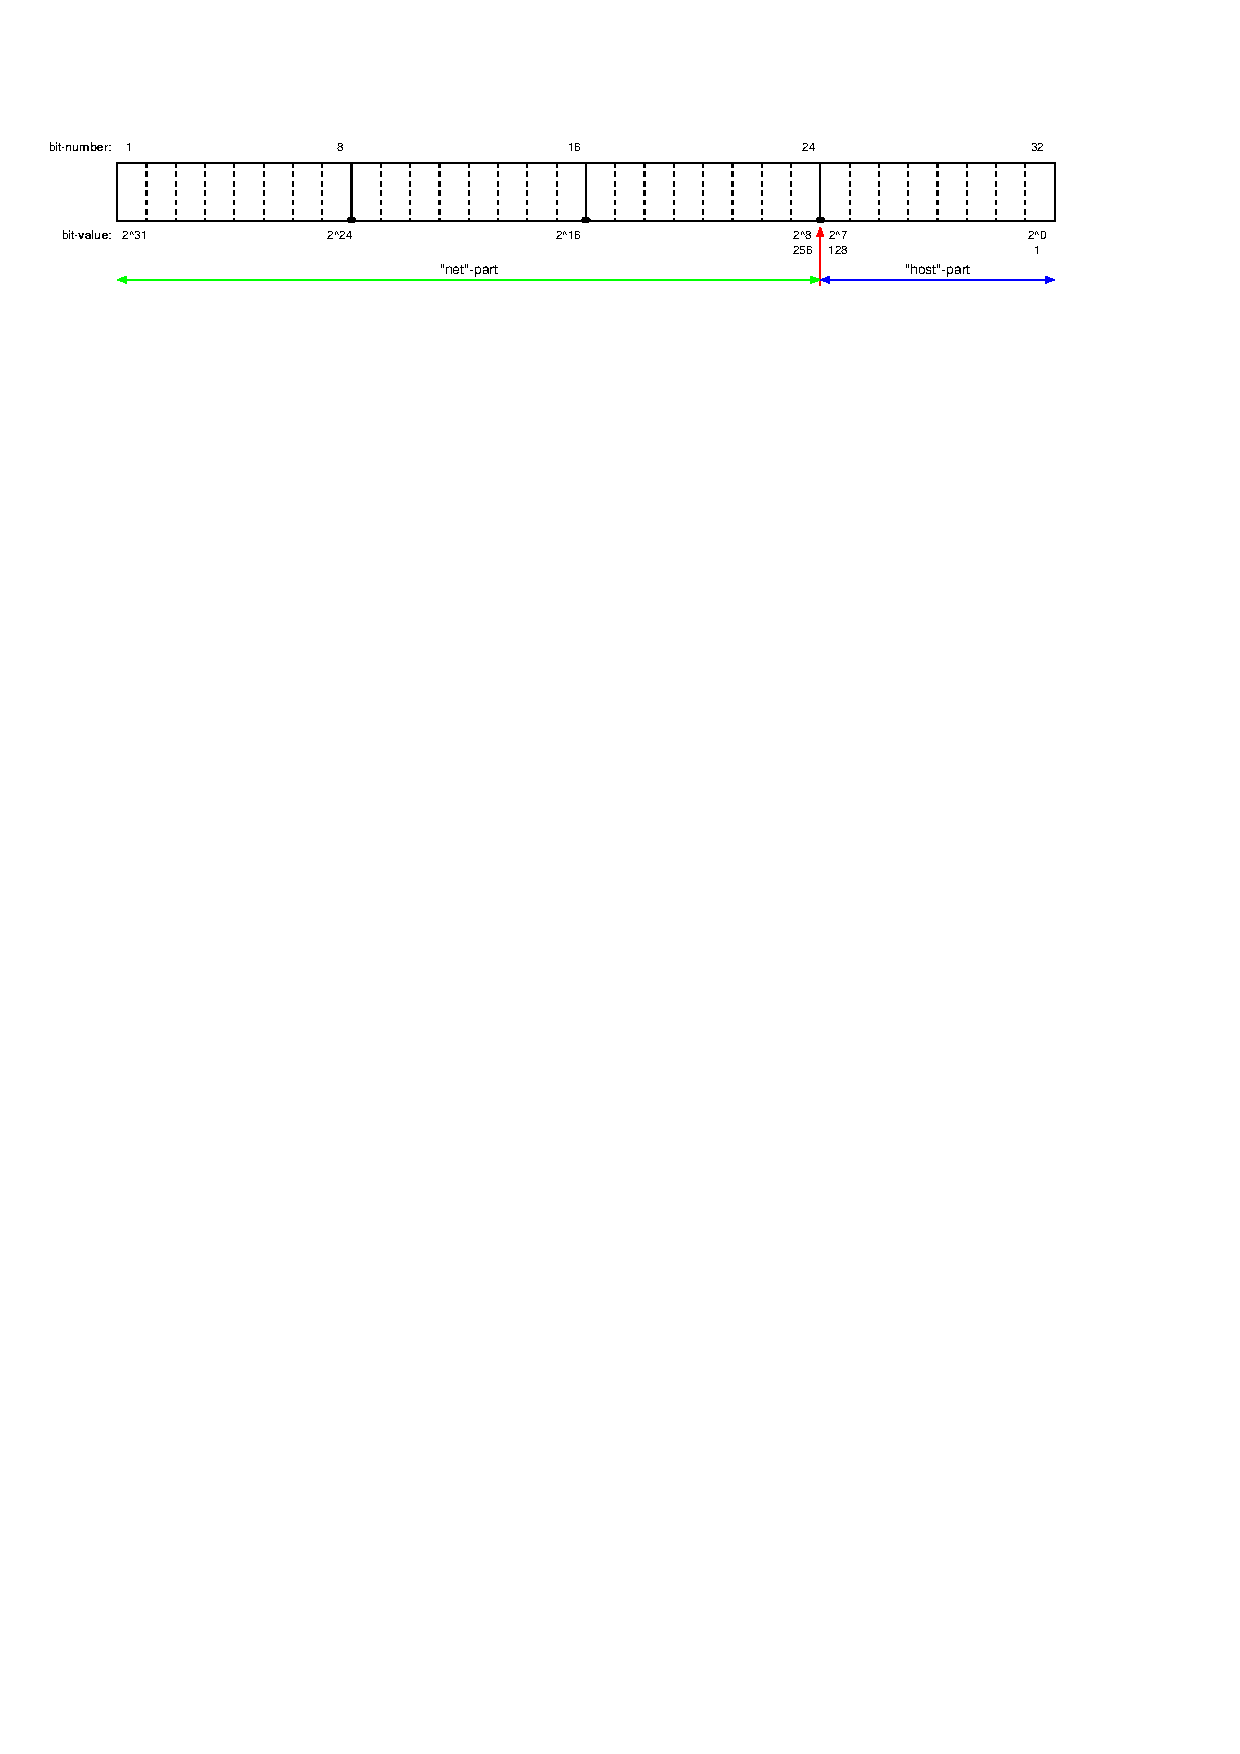
\includegraphics[height=1.6cm]{ip-address}}
\begin{itemize}
	\item{die 32-Bit werden in {\em Netz-} und {\em Host-}Anteil unterteilt\footnote{manchmal zus\"atzlich in Sub-Netz-Anteil}}
	\begin{itemize}
	\item{{\tiny Netz: entspricht etwa Landes-, Ortsvorwahl im Telefonnetz}}
	\item{{\tiny Host: entspricht etwa Nummer des Telefonapparates ohne Vorwahl}}
  \end{itemize}
  \item{Das ``routing''\footnote{Wegleitung} wird aufgrund des Netz-Anteils bestimmt}
  \begin{itemize}
	\item{{\tiny \ldots wie beim Telenfonnetz\ldots}}
\end{itemize}
  \item die Aufteilung ist im Gegensatz zum Telefonsystem in weiten Grenzen anpassbar\footnote{d.h. der Prefix hat nicht eine fest vorgegebene Gr\"osse}
	\end{itemize}
\end{frame}

\begin{frame}
\frametitle{Struktur der IP-Adressen: Prefix-Extraktion (3/3)}
\begin{itemize}
	\item{der Netz-Anteil kann mittels {\em Netzmasken} oder {\em Pr\"afixl\"angen} angegeben werden:}
	\begin{itemize}
	\item{{\tiny bit-and Maske im ``dotted-decimal'' Format: {\textbf {\texttt 255.255.255.0}}, bin\"ar: {\textbf {\texttt 11111111.11111111.11111111.00000000}}}}
	\item{{\tiny Pr\"afixl\"ange (Anzahl gesetzter=``1'' Bits\footnote{``consecutive 1-bits from MSB''} in der Maske): {\textbf {\texttt /24}}}}
\end{itemize}
\item{Netzzugeh\"origkeit: wird mittels der logischen ``Bitwise-And'' Operation durchgef\"uhrt}
\begin{itemize}
	\item{{\tiny IP-Adresse in bin\"ares Format umrechnen, eg: {\texttt 192.168.1.5}$_{10}$$\rightarrow${\texttt 11000000.10101000.00000001.00000101}$_{2}$}}
	\item{{\tiny IP-Maske in bin\"ares Format verwandeln, eg: {\texttt 255.255.255.0}$_{10}$$\rightarrow${\texttt 11111111.11111111.11111111.00000000}$_{2}$}}
	\item{{\tiny ``bitwise-and'' Verkn\"upfung von IP-Adresse und -Maske, eg:\\{\texttt 11000000.10101000.00000001.00000101}$_{2}$ {\textbf \&} {\texttt 11111111.11111111.11111111.00000000}$_{2}$ $=$\\{\texttt 11000000.10101000.00000001.00000{\textbf 0}0{\textbf 0}}$_{2}$ $\rightarrow$ {\texttt 192.168.1.{\textbf 0}}$_{10}$
	}} 
	\item{{\tiny \ldots die so gewonnene Adresse wird als {\em Netzbasisadresse} bezeichnet und kann {\em nicht} f\"ur ein Endger\"at/Node verwendet werden}}
\end{itemize}
\item{der Host-Anteil kann auf gleiche Weise gewonnen werden, wenn die Maske zuerst {\em invertiert}\footnote{``one's-complement''} wird}
\end{itemize}
\end{frame}


\begin{frame}
\frametitle{Interlude}
\begin{itemize}
	\item{finden Sie die IP-Adresse und die Netzmaske Ihres Laptops\footnote{{\texttt ifconfig}/{\texttt ipconfig}, {\texttt netstat -r}}}
	\item{bestimmen Sie aus diesen Informationen die {\em Netzbasisadresse} und den Host-Anteil}
	\item{bestimmen Sie ob die beiden IP-Adressen \texttt{192.168.2.126} und \texttt{192.168.2.130} bei Verwendung einer Netzmaske (f\"ur beide) von \texttt{255.255.255.128} im selben Netz liegen}
	\item{bestimmen Sie die Anzahl m\"oglicher\footnote{Gesamtanzahl minus zwei: broadcast und base} IP-Adressen bei Verwendung der Netzmasken \texttt{255.255.255.0} und \texttt{255.255.254.0}}
	\item{berechnen Sie die ``l\"angste''\footnote{d.h. das eben gerade ausrechende kleinste Netzwerk} Netzmaske wenn rund 2000 Adressen im selben Netz ben\"otigt werden}
\end{itemize}
\end{frame}


\begin{frame}
\frametitle{Aufteilung des Adressbereichs}
\begin{itemize}
  \item{bis ca 1993 ``chaotisch'': \myurl{http://www.iana.org/assignments/ipv4-address-space/ipv4-address-space.xml}}
  \item{seither (CIDR) in geographisch/institutionell hierarchischer Weise \"uber ``Unterverteiler'' RIR\footnote{regional-internet-registry, z.B. \myurl{http://www.ripe.net/}}, private Provider\footnote{z.B. 212.x.x.x und 213.x.x.x sind beide ``Europa'' -- \"ahnlich wie ``Landesvorwahl''}}
\end{itemize}
\end{frame}


\begin{frame}
\frametitle{IP-Adressbereich als Klassen ``{\Huge {\frakfamily ye olde way}}'' 1/2}
\begin{center}
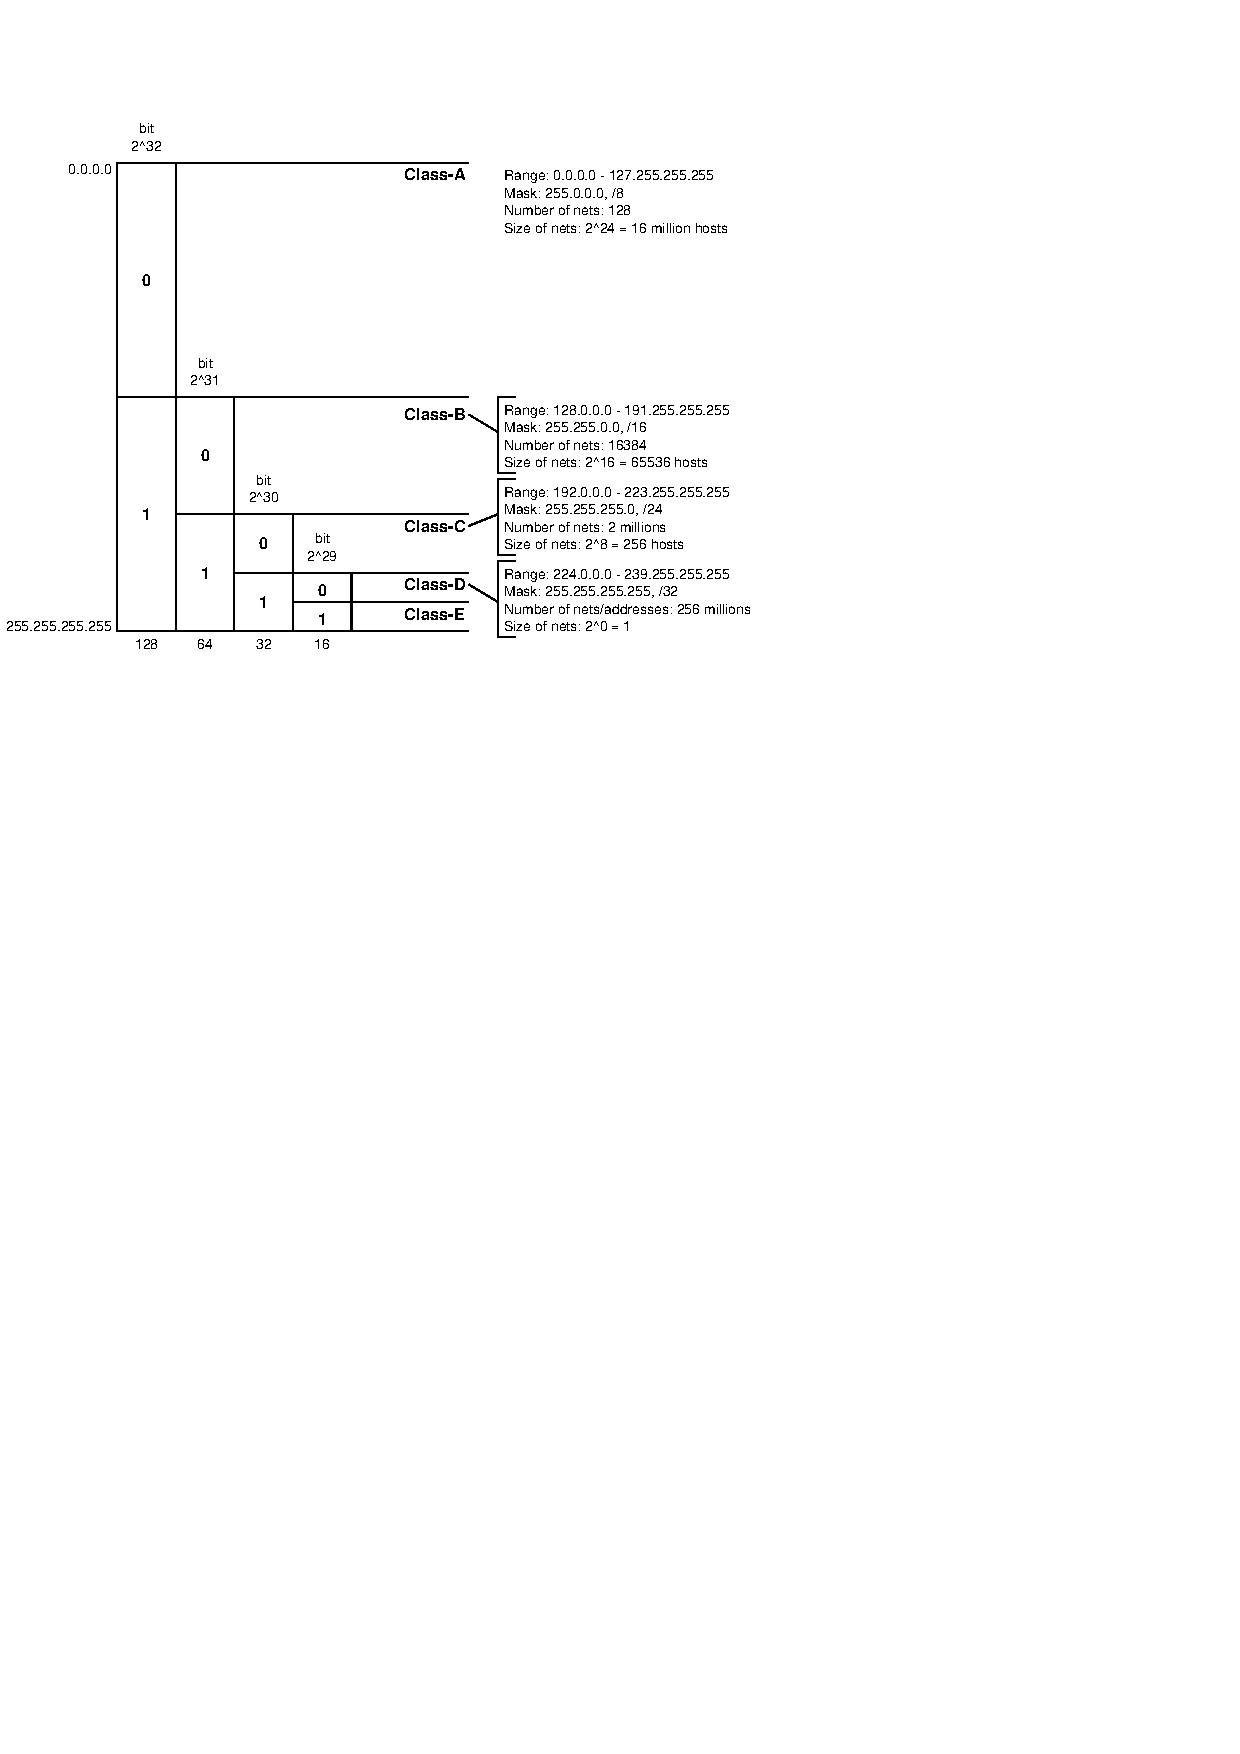
\includegraphics[height=21cm]{class-based}
\end{center}
\end{frame}

\begin{frame}
\frametitle{IP-Adressbereich als Klassen ``{\Huge {\frakfamily ye olde way}}'' 2/2}
\begin{itemize}
	\item{es werden mit {\em ID-Bits} identifizierte Adressbereiche f\"ur grosse, mittlere und kleine Netze gebildet}
	\item{\ldots ``it seemed a good idea in the 80\'{}''}
	\item{Problem-1: nur 128 Netze belegen die H\"alfte des Addressraums (aber k\"onnen 16 Millionen Hosts aufnehmen)}
	\item{Problem-2: keine topographisch/hierarchische\footnote{wie z.B. das Telefonnetz} Aufteilung}
	\item{Problem-3\footnote{big, fat\ldots}: Router m\"ussen im schlechtesten Fall etwas \"uber {\em 2 Millionen} Netze kennen}
\end{itemize}
\end{frame}

\begin{frame}
\frametitle{CIDR ``Classless Inter-Domain Routing'' (the new way) 1/2}
\begin{itemize}
	\item{Neustrukturierung\footnote{soweit m\"oglich\ldots Bereits zugewiesene Netze k\"onnen nicht entfernt werden} des Adressbereichs}
	\item{Klassen werden {\em nicht} mehr beachtet}
	\item{Bildung von {\em Supernetzen} f\"ur effizientes hierarchies routing\footnote{eg. {\texttt 212/7$\rightarrow$Europa}}\\$\rightarrow$ kleine Routing-Tables}
	\item{Bessere Ausnutzung des Adressbereichs durch Aufteilung der A- und B-Klassen in kleinere Einheiten}
  \item{{\bfseries neue Notation} als {\em Pr\"afixl\"ange}\footnote{``slash''-Notation}: {\texttt 255.255.240.0}$\rightarrow${\texttt /20}}
\end{itemize}
\end{frame}

\begin{frame}
\frametitle{CIDR ``Classless Inter-Domain Routing'' (the new way) 2/2}
\begin{center}
\includegraphics[height=5.5cm]{bgp-growth.pdf}
\end{center}
{\tiny \verbatiminput{bgp-table-growth.sh}}
\end{frame}

\begin{frame}
\frametitle{\ldots noch mehr Spass mit Bits}
\begin{itemize}
\item{Berechnen Sie zu der CIDR-Pr\"afixl\"ange \texttt{/20} die entsprechende Netzmaske}
\item{\ldots und umgekehrt zu der Netzmaske \texttt{255.255.192.0} die Pr\"afixl\"ange}
\item{wieviele m\"ogliche IP-Adressen k\"onnen in \texttt{/21} untergebracht werden?}
\item{Bestimmen Sie ob die beiden IP-Adressen \texttt{172.17.71.5/23} und \texttt{172.17.70.240} im selben Netz liegen}
\end{itemize}
\end{frame}



\begin{frame}
\frametitle{Reservierte/Spezielle IP-Prefix/Adressen}
einige Bereiche im IP-Adressraum sind reserviert:
\begin{small}
\begin{center}
\begin{tabular}{|c|l|l|}
\hline 
\textbf{IP} & \textbf{Bedeutung} & \textbf{Source/Destination} \\
0.0.0.0 & unbekannte Source \tiny{(DHCP/BOOTP)} & nur Source \\
255.255.255.255 & limited Broadcast & nur Destination\tiny{, stoppt am Router} \\
127.0.0.0/8 & loopback\tiny{, Host-lokal} & beides, nur Host-intern \\
192.168.0.0/16 & {\em private} IP\tiny{, RFC1918, braucht NAT f\"ur Internet} & beides\tiny{, wird im Internet nicht geroutet} \\
172.16.0.0/12 & {\em private} IP\tiny{, RFC1918, braucht NAT f\"ur Internet} & beides\tiny{, wird im Internet nicht geroutet} \\
10.0.0.0/8 & {\em private} IP\tiny{, RFC1918, braucht NAT f\"ur Internet} & beides\tiny{, wird im Internet nicht geroutet} \\
169.254.0.0/16 & Link-Local\tiny{, automatisch IPs ohne DHCP} & beides\tiny{, wird im Internet nicht geroutet} \\
\hline
10.195.5.0/24 & Netz-Basisadresse\tiny{, alle Hostbits=0} & keine \\
10.195.5.255/24 & directed Broadcast\tiny{, alle Hostbits=1} & nur Destination \\
\hline 
\end{tabular}
\end{center}
\end{small}
\myurl{http://www.inetdaemon.com/tutorials/internet/ip/addresses/special.shtml}\\
\myurl{http://de.wikipedia.org/wiki/IP-Adresse\#Besondere_IP-Adressen}\\
\myurl{http://www.rfc-editor.org/rfc/pdfrfc/rfc1918.txt.pdf}
\end{frame}

%\begin{frame}
%\frametitle{Routing und Routing-Table}
%\begin{itemize}
%	\item{die Wegleitung ``routing'' im Internet:}
%	\begin{itemize}
%	\item{{\tiny wird bei jedem Router\footnote{``hop-by-hop'' und ``next-hop''} neu entschieden und dann an den n\"achsten Router oder an den Zielhost zugestellt}}
%	\item{{\tiny entschieden wird der ``next-hop'' \"uber die {\em Routing-Tabelle}\footnote{im Folgdenen ``routing-table'' oder RT -- eigentlich ist das die FIB}}}
%	\item{{\tiny der Ablauf wird f\"ur jedes Paket neu gemacht}}
%\end{itemize}
%\item{die {\em Routing-Tabelle} enth\"alt (mindestens):}
%\begin{itemize}
%	\item{{\tiny {\em Ziel-Netz} (dest-net)}}
%	\item{{\tiny {\em Ziel-Maske} oder {\em Ziel-Pr\"afixl\"ange} (dest-mask, prefixlength)}}
%	\item{{\tiny {\em N\"achster-Router} (next-hop oder gateway)}}
%\end{itemize}
%\item{der {\em Routing-Vorgang} (forwarding): findet den ``next-hop'' f\"ur eine gegeben/empfangene IP-{\em Ziel}-Adresse (target-ip)}
%\begin{itemize}
%	\item{RT-Eintrag ``passt'', wenn: \\{\texttt ( target-ip {\textbf \&} dest-mask$_{i}$ ) = dest-net$_{i}$}, dann wird das Paket an {\texttt next-hop$_{i}$} weitergeleitet}
%	\item{die RT wird nach Pr\"afixl\"ange in {\em absteigender} Reihenfolge konsultiert}
%	\item{die ``Default-Route'' ist \texttt{0.0.0.0/0}}
%\end{itemize}
%\end{itemize}
%\end{frame}


\begin{frame}
\frametitle{Routing und Routing-Table (1/3)}
die Wegleitung -- {\em routing} -- im Internet:
	\begin{itemize}
	\item{{\em Router} empfangen Pakete und leiten sie in Richtung Zieladresse\footnote{aus dem Paketinhalt/Layer-3 Adresse} weiter: {\em routing} oder {\em forwarding}}
	\item{jedes Paket wird gesondert betrachtet\footnote{wichtig um die Robustheit des paketvermittelnden Netzes zu gew\"ahrleisten (moderne Router arbeiten m\"oglicherweise effizienter)}}
	\item{Pakete werden an den jeweils n\"achsten Router -- {\em next-hop} -- gesendet}
	\item{der ``letzte Router''\footnote{Router-Interface ist im selben Netzwerk wie die Zieladresse} stellt das Paket direkt an den Zielknoten\footnote{Endger\"at, der Router findet die L2-Adresse mittels ARP} zu}
	\item{entschieden wird das alles \"uber die {\em Routing-Tabelle}}
\end{itemize}
\end{frame}

\begin{frame}
\frametitle{Routing und Routing-Table (2/3)}
die {\em Routing-Tabelle} (RT) enth\"alt (mindestens):
\begin{itemize}
	\item{{\em Ziel-Netz} {\small (``dest-net'' oder einfach ``net'')}}
	\item{{\em Ziel-Maske} oder {\em Ziel-Pr\"afixl\"ange} {\small (``dest-mask'', ``prefixlength'', ``prefix'')}}
	\item{{\em N\"achster-Router} {\small (``next-hop'' oder ``gateway'')}}
	  %%\item{\includegraphics{routing-table}}
\end{itemize}
\begin{tiny}
Beispiele:
\verbatiminput{routingtable.txt}
\end{tiny}
\end{frame}

\begin{frame}
\frametitle{Routing und Routing-Table (3/3)}
Ablauf ``forwarding'' -- Paket weiterleiten
\begin{itemize}
  \item{finde passenden RT-Eintrag zur Zieladresse des weiterzuleitenden Pakets -- f\"ur jede Zeile \texttt{$j$} der RT:
    \\ {\texttt target-ip \textbf{$\wedge$} dest-mask$_{j}$ = dest-net$_{j}$}}
  \item{falls ein passender Eintrag gefunden wurde, wird das Paket als Frame zur L2-Adresse der L3-Adresse \textbf{\texttt{next-hop$_{j}$}} weitergeleitet}
  \item{falls der Router selbst eine IP-Adresse/Interface im Ziel{\em netz} hat, wird das Frame direkt an das Endger\"at zugestellt}
	\item{die Routing-Tabelle wird nach absteigender\footnote{von ``spezifisch'' zu ``allgemein''} Pr\"afixl\"ange abgearbeitet/sortiert}
	\item{die {\em Default-Route}\,\footnote{``passt'' immer und wird am Schluss abgearbeitet} ist {\texttt 0.0.0.0/0}}
\end{itemize}
\end{frame}

\begin{frame}
\frametitle{Intermezzo}
Tools zum Thema
\begin{itemize}
	\item{\textbf{\texttt{netstat -rn}} zeigt lokale Routing-Tabelle an $\rightarrow$ finden des ``Default-Router''}
	\item{\textbf{\texttt{arp -a}} zeigt die lokale ARP-Tabelle an $\rightarrow$ zur Kontrolle der Layer-2/MAC-Adresse des Routers}
	\item{\textbf{\texttt{traceroute}}\footnote{Windows: \texttt{tracert}} (unzuverl\"assiger) {\em Hin}weg\footnote{zeigt die Router an, \"uber die ein Paket wahrscheinlich weitergeleitet wird} zu einer bestimmten L3-Zieladresse}
\end{itemize}
\end{frame}



\begin{frame}
\frametitle{References}
\begin{itemize}
	\item{\myurl{http://en.wikipedia.org/wiki/IPv4_subnetting_reference}}
	\item{\myurl{http://en.wikipedia.org/wiki/Classless_Inter-Domain_Routing}}
	\item{Route-servers: \myurl{http://www.traceroute.org/\#Route\%20Servers}}
	\item{BGP-routing-table growth: \myurl{http://bgp.potaroo.net/as2.0/bgp-active.html}, andere lustige Informationen: \myurl{http://bgp.potaroo.net/as2.0/}}
	\item{CIDR: \myurl{http://books.google.ch/books?id=axiW1d8GosIC\&lpg=PA125\&pg=PA101\#v=onepage\&q=\&f=false}}
	\item{IP-address landscape: \myurl{http://xkcd.com/195/}}
\end{itemize}
\end{frame}



\begin{frame}
\frametitle{ARP: Address Resolution Protocol, (1/2)}
\begin{itemize}
  \item{ARP findet zu einer gew\"unschten IP-Adresse die entsprechende MAC-Adresse: L3?$\rightarrow$L2 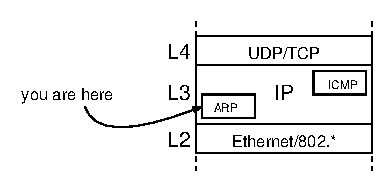
\includegraphics[height=1.5cm]{arp-layer}}


  \item{RARP ist das ``R\"uckw\"artsprotokoll'': 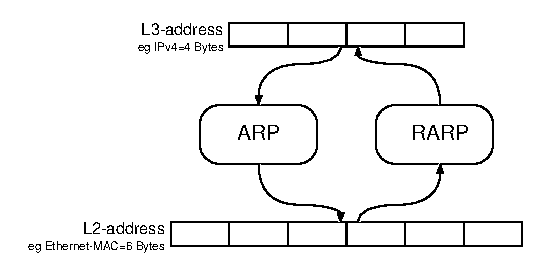
\includegraphics[height=1.5cm]{arp-opschema}}
  \item{ARP und RARP arbeiten beide mit L2/MAC-Broadcasts f\"ur die Anfragen und L2-Unicast f\"ur die Antworten\footnote{\ldots meistens. Deshalb sehen Sie mit \texttt{tcpdump} nur die ARP-Anfragen (Broadcast)}}
\end{itemize}
\begin{tiny}
\verbatiminput{arp-tcpdump.txt}
\end{tiny}
\end{frame}

\begin{frame}
\frametitle{ARP: Address Resolution Protocol, (2/2)}
\begin{itemize}
  \item{Ablauf und Kommunikation} \vspace{0.25cm}
  \begin{figure}{}
     \begin{subfigure}{}
        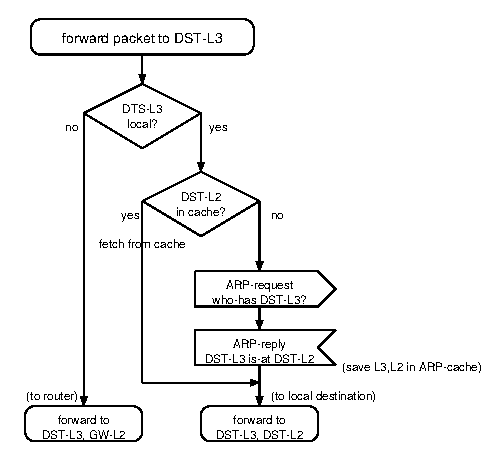
\includegraphics[width=5cm]{arp-procedure.eps}
     \end{subfigure}
     ~
     \begin{subfigure}{}
        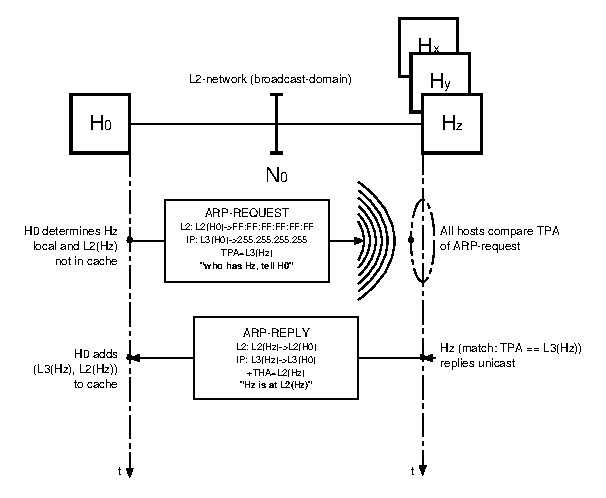
\includegraphics[width=5cm]{arp-communication}
     \end{subfigure}
  \end{figure}
  \item{Tools: ARP-Cache angucken, l\"oschen oder statische Eintr\"age einf\"ugen: \texttt{arp}, \texttt{ip neighbor}}
\end{itemize}
\end{frame}



\begin{frame}
\frametitle{ICMP, Internet Control Message Protocol, (1/3)}
IP (Layer-3) ist {\em best-effort}{}\footnote{Pakete k\"onnen verloren gehen}, d.h. es wird ein Mechanismus zur Fehlersignalisation ben\"otigt: 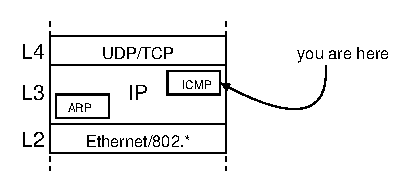
\includegraphics[height=1.5cm]{icmp-layer}
\begin{itemize}
  \item{ICMP implementiert {\em Fehlermeldungen} und {\em Statusabfragen} in TCP/IP}
  \item{Router k\"onnen durch ICMP Fehlerindikationen an das sendende Ger\"at zukommen lassen\footnote{\ldots normalerweise sind Router ``stumm'', resp. d\"urfen nicht in die Kommunikation eingreifen}}
  \item{Die Meldungen sind mit einem Code/Bedeutung markiert und enthalten den Original IP-Header des verursachenden Pakets\footnote{um dem Ger\"at die Zuweisung des Fehlers an das betroffene Programm zu erm\"oglichen (z.B. browser)}}
  \item{bei den meisten Fehlermeldungen wird das Original-Paket verworfen, der Sender muss versuchen es erneut zuzustellen oder die Fehlermeldung an die Applikation weiterzuleiten}
\end{itemize}
\end{frame}

\begin{frame}
\frametitle{ICMP, Internet Control Message Protocol, (2/3)}
\begin{itemize}
	\item{Fehlermeldungen: erm\"oglicht Router und Endger\"ate die Paketquelle \"uber Fehler zu informieren (Auswahl)\\   \begin{tiny}
	    \begin{tabular}{|l|l|l|l|}
	      \hline
	      \textbf{Meldung} & \textbf{Bedeutung} & \textbf{Sender} & Verworfen \\
	      \hline
	      network unreachable & kein passender Routing-Table Eintrag & Router & Paket verworfen \\
	      host unreachable & keine Antwort auf ARP & letzter Router & Paket verworfen \\
	      port unreachable & kein Serverprozess, Listen-Socket & Zielhost & Paket verworfen \\
	      time exceeded & TTL abgelaufen\footnote{{\em Time To Live} ist ein numerisches Feld im IP-Header und wird von jedem Router dekrementiert (-1) -- bei 0 $\rightarrow$ time-exceeded} & Router & Paket verworfen \\
	      fragmentation needed & Paket zu gross & Router & Paket verworfen \\
	      redirect & an anderen Router senden\footnote{enth\"alt IP des ``besseren'' Routers $\rightarrow$ Routing-Table} & Router & Paket weitergeleitet \\
	      source-quench & Flusskontrolle, veraltet\footnote{\ldots da meistens ignoriert und zus\"atzlicher Aufwand (Status) f\"ur Router} & Router & Paket weitergeleitet \\
	      \hline
	    \end{tabular}
	  \end{tiny}
	}
	\vspace{0.25cm}
	\item{Statusabfragen: erm\"oglicht einfache Statusabfragen auf Layer-3}\\    \begin{tiny}
	    \begin{tabular}{|l|l|l|}
	      \hline
	      \textbf{Meldung} & \textbf{Bedeutung} & \textbf{Sender} \\
	      \hline
				echo-request und echo-reply & Erreichbarkeitstest\footnote{z.B. \texttt{ping}} auf Layer-3 & alle \\
				timestamp-request und -reply & Zeitstempel\footnote{enth\"alt Local-Absende-, Remote-Empfangs- und Absende-Zeitstempel. Local-Empfangszeitstempel wird bei Erhalt der -reply-Meldung eingetragen} Abfrage & alle \\
	      \hline
	    \end{tabular}
	  \end{tiny}
\end{itemize}
\end{frame}


\begin{frame}
\frametitle{ICMP, Internet Control Message Protocol, (3/3)}
{\center 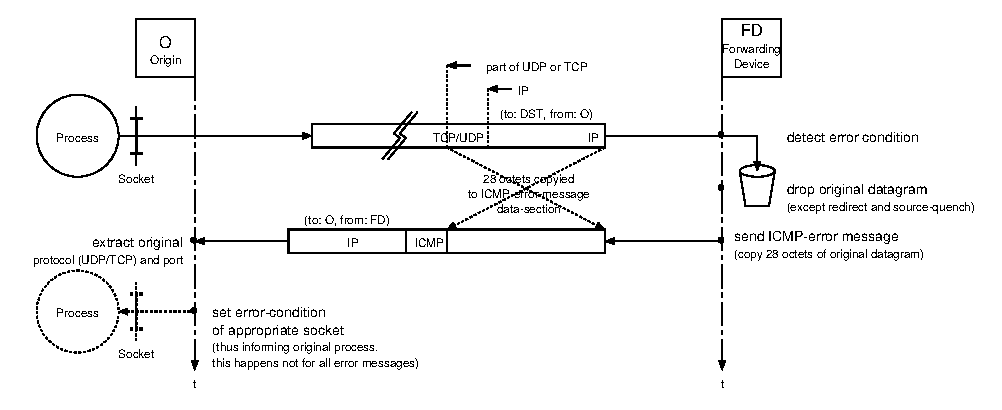
\includegraphics[height=5cm]{icmp-errormessage}} \\
{\center 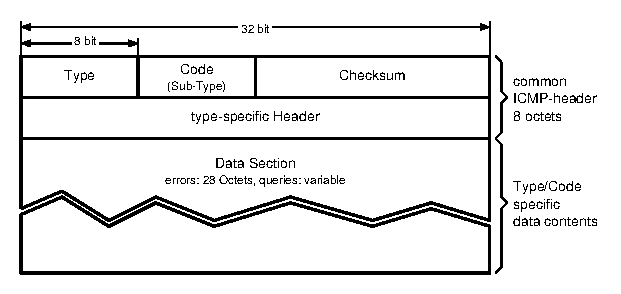
\includegraphics[height=2cm]{icmp-packetformat}}
\end{frame}

\begin{frame}[fragile]
\frametitle{ICMP Tools (1/2)}
\begin{itemize}
	\item{\textbf{\texttt{ping}}: Layer-3 reachability} testen Erreichbarkeit\footnote{mit Hilfe von ICMP-echo-request Meldungen} auf Layer-3:
		\begin{tiny}
		\begin{verbatim}
rschmutz@callisto ~ $ ping -c 3 www.google.ch
PING www.l.google.com (209.85.227.99): 56 data bytes
64 bytes from 209.85.227.99: icmp_seq=0 ttl=54 time=44.935 ms
64 bytes from 209.85.227.99: icmp_seq=1 ttl=54 time=41.854 ms
64 bytes from 209.85.227.99: icmp_seq=2 ttl=54 time=58.240 ms

--- www.l.google.com ping statistics ---
3 packets transmitted, 3 packets received, 0.0% packet loss
round-trip min/avg/max/stddev = 41.854/48.343/58.240/7.110 ms
\end{verbatim}
\end{tiny}
\item{\texttt{ping}/ICMP-Echo-Request testet nur die \emph{Erreichbarkeit auf Schicht-3 ``End-zu-end System''}\footnote{d.h. IP-Adresse/Host kann erreicht werden aber keine Angaben \"uber die Verf\"ugbarkeit eines speziellen Dienstes (Mail, Web, etc) auf diesem Host}}
\item{ICMP-Echo-Request/Response wird h\"aufig auf Firewalls ``geblockt''
  \begin{itemize}
    \item{\texttt{ping} auf eine Adressen/Host ergibt keine Antwort (timeouts) \emph{aber} der HTTP-Dienst auf derselben Adresse/Host ist verf\"ugbar\footnote{z.B. \texttt{ping www.microsoft.com}$\rightarrow$nix aber \texttt{http://www.microsoft.com/} im Browser funktioniert}}
  \end{itemize}
}
\item{die Ausgabe ist normalerweise die ``Round-Trip-Time'', d.h. die total ben\"otigte Zeit Anfrage+Verarbeitung+Antwort}
\end{itemize}
\end{frame}


\begin{frame}[fragile]
\frametitle{ICMP Tools (2/2)}
\begin{itemize}
	\item{\textbf{\texttt{traceroute}}: Layer-3 route path\footnote{durch erzwingen von 		ICMP-time-exceeded und ICMP-port-unreachable Meldungen}}
\begin{tiny}
		\begin{verbatim}
rschmutz@zaphod:~$ traceroute www.google.com
traceroute to www.google.com (209.85.135.103), 30 hops max, 40 byte packets
 1  static.193.65.40.188.clients.your-server.de (188.40.65.193)  0.676 ms  0.702 ms  0.723 ms
 2  hos-tr1.juniper1.rz10.hetzner.de (213.239.227.129)  0.189 ms  0.194 ms
    hos-tr4.juniper2 (213.239.227.225)  0.178 ms
 3  hos-bb1.juniper2.ffm.hetzner.de (213.239.240.226)  4.559 ms  4.576 ms  4.597 ms
 4  de-cix10.net.google.com (80.81.192.108)  5.682 ms  5.981 ms  6.331 ms
 5  209.85.255.172 (209.85.255.172)  6.098 ms
    209.85.255.170 (209.85.255.170)  16.070 ms  6.192 ms
 6  72.14.238.128 (72.14.238.128)  14.460 ms  14.001 ms
    209.85.248.248 (209.85.248.248)  11.706 ms
 7  209.85.241.187 (209.85.241.187)  13.981 ms
    209.85.241.83 (209.85.241.83)  13.886 ms  14.033 ms
 8  209.85.253.22 (209.85.253.22)  13.074 ms  13.896 ms
    72.14.239.54 (72.14.239.54)  27.321 ms
 9  mu-in-f103.1e100.net (209.85.135.103)  15.272 ms  15.526 ms  13.659 ms
\end{verbatim}
\end{tiny}
\begin{small}
\item{\texttt{traceroute} zeigt den scheinbaren ``Pfad''\footnote{IP=Paketvermittelnd $\rightarrow$ \emph{kein} ``Pfad'', d.h. \texttt{traceroute} l\"ugt ein bisschen} -- d.h. die einzelnen Router + Distanz in ``hops'' -- zu einer Zieladresse}
\item{dazu werden TTL-begrenzte Pakete\footnote{z.B. UDP-Pakete an m\"oglichst unbenutzte Ports} ausgesendet und die ICMP-Time-Exceeded-in-Transit Meldungen der Router ausgegeben}
\item{wie auch \texttt{ping} wird \texttt{traceroute} h\"aufig ``geblockt'' und zudem sind die Angaben interpretationsbed\"urftig}
\end{small}
\end{itemize}
\end{frame}


\end{document} 
